\section{MPI One-Sided Communication}
\subsection{Required submission files}
\begin{enumerate}
  \item \hl{The updated \emph{gauss.c} file.}

    \verb!Data/path/to/file!

  \item \hl{The new performance plots and description in the report.}

    References to figures here...

\end{enumerate}

\subsection{Questions}
\begin{enumerate}
  \item \hl{Which one-sided operations were used? Justify your choice.}

    We have decided to use \verb!MPI_Win_start!, \verb!MPI_Win_post!, \verb!MPI_Get! and \verb!MPI_Win_complete!.
    We have decided to go with \verb!MPI_Get! function because it fits the purpose of distributing
    data from the process that had computed his part of pivoting to the rest.

  \item \hl{Was communication and computation overlap achieved? Use Vampir.}

    Yes it was achieved and it can be seen in Fig \todo{Put image of vampir}

  \item \hl{Was a speedup observed versus the baseline for the Sandy Bridge and Haswell nodes?}

    Results performed on Haswell and Sandy Bridge for One sided communication are almost the same.
  
    Despite the fact that overlap of the communication and computation was achieved, overall time
    was even worth than for baseline. This was due the fact that processors with higher 
    IDs that process were slower in processing their part. Therefore they become a bottleneck
    for this implementation.

  \item \hl{Was a speedup observed versus the non-blocking version for the Sandy Bridge and Haswell nodes?}

    \todo{Wait for results of non-blocking}

\end{enumerate}
% % Figure example
% \begin{figure}[p] % h=here, t=top, b=bottom, p=(extra)page, !=force
%    \begin{center}
%      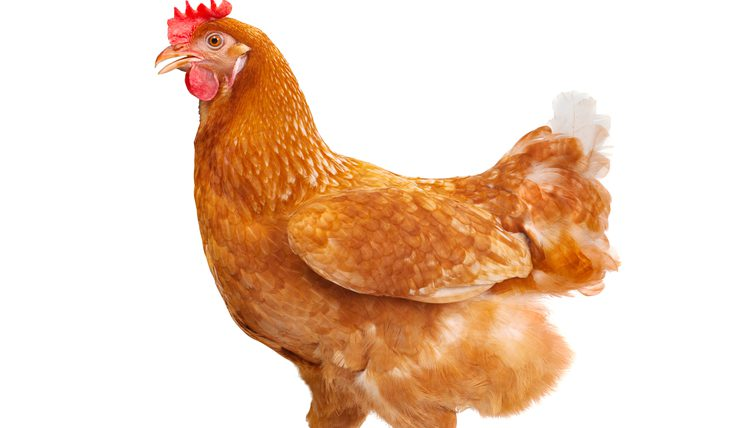
\includegraphics[width=.9\linewidth]{figure.png} % It searches in the Figures/ folder!
%      \caption{Caption text}
%      \label{fig:figureLabelName}
%    \end{center}
% \end{figure}
